\documentclass[10pt]{beamer}

% Beamer style
%\usetheme[secheader]{Madrid}
% \usetheme{CambridgeUS}
\useoutertheme{infolines}
\usecolortheme[rgb={0.65,0.15,0.25}]{structure}
%\usefonttheme[onlymath]{serif}
\beamertemplatenavigationsymbolsempty
%\AtBeginSubsection

% Packages
%\usepackage[french]{babel}
\usepackage[latin1]{inputenc}
\usepackage{color}
\usepackage{dsfont, stmaryrd}
\usepackage{amsmath, amsfonts, amssymb}
\usepackage{stmaryrd}
\usepackage{epsfig}
\usepackage{/home/robin/LATEX/Biblio/astats}
%\usepackage[all]{xy}
\usepackage{graphicx}

% Commands
\definecolor{darkred}{rgb}{0.65,0.15,0.25}
\definecolor{darkgreen}{rgb}{0,0.4,0}
\newcommand{\emphase}[1]{\textcolor{darkred}{#1}}
%\newcommand{\emphase}[1]{\textcolor{black}{#1}}
\newcommand{\paragraph}[1]{\textcolor{darkred}{#1}}
\newcommand{\refer}[1]{\textcolor{gray}{\footnotesize [\cite{#1}]}}
\newcommand{\Refer}[1]{\textcolor{gray}{\footnotesize [#1]}}
% \newcommand{\newblock}{}


%====================================================================
%====================================================================
\title{HMM for tiling array analysis: ChIP-chip and transcriptome}

\author{C. B�rard, MLMM, TMH, SR, SV}

\date{}

%====================================================================
%====================================================================
\begin{document}
%====================================================================
%====================================================================

%====================================================================
\maketitle

%====================================================================
\frame{\frametitle{Tiling arrays} 
  $$
  \begin{array}{c}
  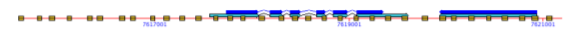
\includegraphics[width=.9\textwidth]{../FIGURES/Ber12-Fig1-11} \\
  \pause ~\\ 
  \hline
  ~\\
  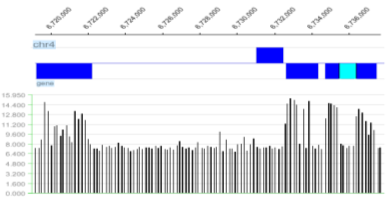
\includegraphics[width=.7\textwidth]{../FIGURES/Ber12-Fig1-10}
  \end{array}
  $$
  }

%====================================================================
\frame{\frametitle{ChIP-chip data} 
  $$
  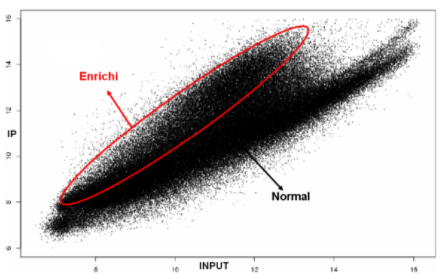
\includegraphics[width=.8\textwidth]{../FIGURES/Ber12-Fig3-3}
  $$
  }

%====================================================================
\frame{\frametitle{Mixture model} 
  $$
  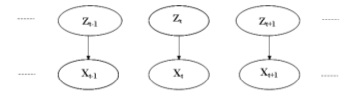
\includegraphics[width=.8\textwidth]{../FIGURES/Ber12-Fig2-2}
  $$
  ~\\
  $t = $ probe number or location \\
  ~\\
  $Z_t =$ hidden status: 1 if epigenetic signal, 0 otherwise \\
  ~\\
  $X_t =$ observed signal: $X_t = (IP_t, Input_t)$
  }

%====================================================================
\frame{\frametitle{Bivariate observation: $X_t = (IP_t, Input_t)$} 
  $$
  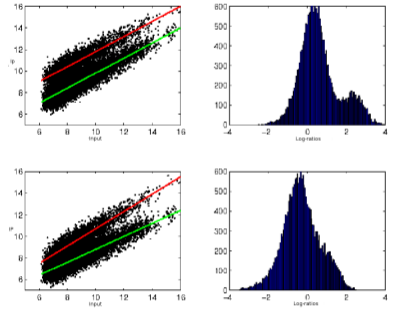
\includegraphics[width=.7\textwidth]{../FIGURES/Ber12-Fig3-4}
  $$
  }

%====================================================================
\frame{\frametitle{Working on emission distributions} 
  $$
  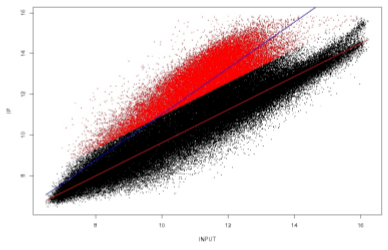
\includegraphics[width=.7\textwidth]{../FIGURES/Ber12-Fig5-6}
  $$
  \begin{eqnarray*}
   IP_t & = & a_0 + b_0 Input_t + E_t \qquad \text{if } Z_t = 0 \\
   & & a_1 + b_1 Input_t + E_t \qquad \text{if } Z_t = 1 \\
  \end{eqnarray*}
  }

%====================================================================
\frame{\frametitle{Comparison the Nimblegene sofware} 
  $$
  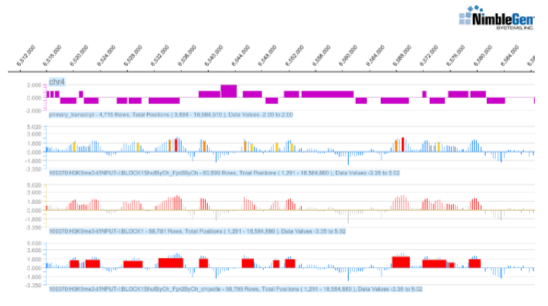
\includegraphics[width=.8\textwidth]{../FIGURES/Ber12-Fig5-8}
  $$
  1 = annotation, 2 = Nimblegene peak detection, 3 = enriched probes according to ChIPmix, 4 = regions detected by ChIPotle
  }

%====================================================================
\frame{\frametitle{Hidden Markov model (HMM)} 
  $$
  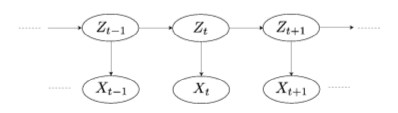
\includegraphics[width=.8\textwidth]{../FIGURES/Ber12-Fig2-3}
  $$
  ~\\
  $t = $ probe number or location \\
  ~\\
  $Z_t =$ hidden status: 1 if epigenetic signal, 0 otherwise \\
  ~\\
  $X_t =$ observed signal
  }

%====================================================================
\frame{\frametitle{HMM with annotation} 
  $$
  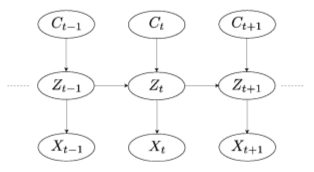
\includegraphics[width=.6\textwidth]{../FIGURES/Ber12-Fig3-2}
  $$
  $C_t=$ annotation, $X_t=$ observed signal, $Z_t=$ hidden status \\
  ~\\  
  $X_t = (IP_t, Input_t)$ or $X_t = (IP^A_t, IP^B_t)$
  }

%====================================================================
\frame{\frametitle{Comparing two conditions} 
  $$
  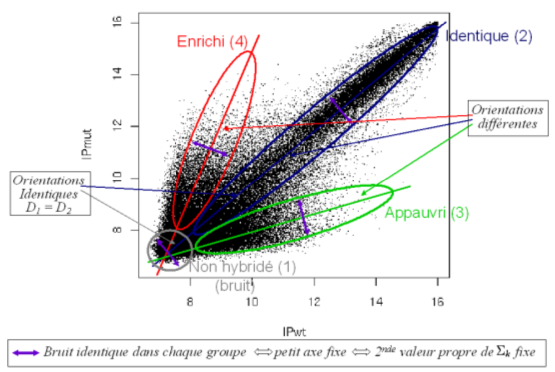
\includegraphics[width=.8\textwidth]{../FIGURES/Ber12-Fig3-8}
  $$
  }

%====================================================================
\frame{\frametitle{Fit of the emission distribution} 
  $$
  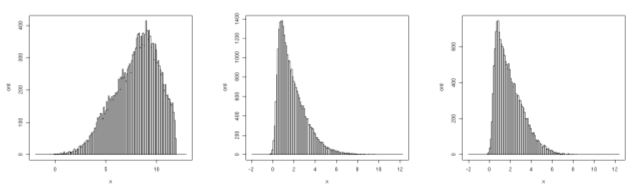
\includegraphics[width=.8\textwidth]{../FIGURES/Ber12-Fig3-9}
  $$
  Do not look Gaussian
  }

%====================================================================
\frame{\frametitle{Emission distribution = mixture} 
  $$
  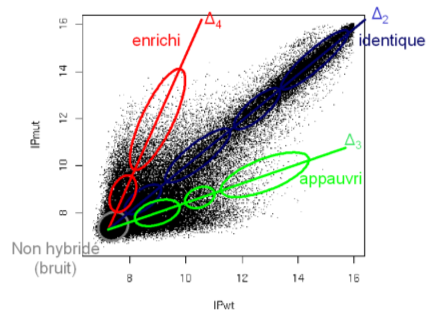
\includegraphics[width=.7\textwidth]{../FIGURES/Ber12-Fig3-10}
  $$
  }

%====================================================================
\frame{\frametitle{Non-parametric emission distribution (kernel estimate)} 
  $$
%   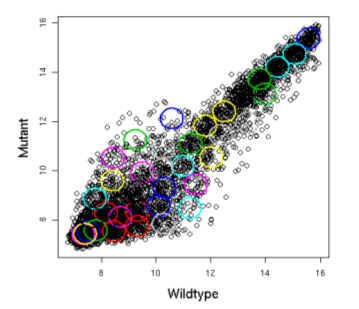
\includegraphics[width=.6\textwidth]{../FIGURES/Ber12-Fig3-11}
  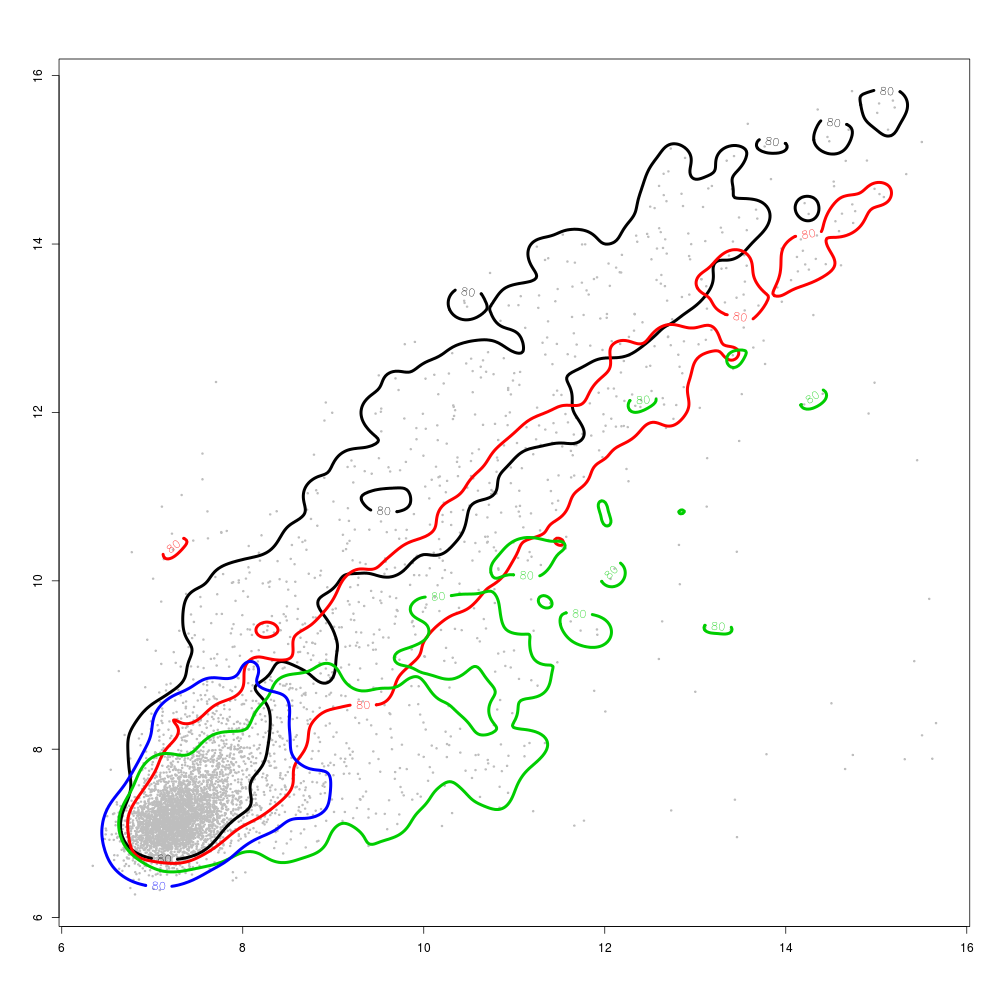
\includegraphics[width=.6\textwidth]{../FIGURES/data1_10dap_5000-K4-bw0_139551228238152}
  $$
  }

%====================================================================
\frame[allowframebreaks]{ \frametitle{References}
{\tiny
  \nocite{MMB08,BMB11,RAB11,VBM13}
  \bibliography{/home/robin/Biblio/AST}
  \bibliographystyle{plain}
  }
}


%====================================================================
%====================================================================
\end{document}
%====================================================================
%====================================================================


\begin{tabular}{cc}
 \begin{tabular}{p{.5\textwidth}}
 \end{tabular}
 &
 \hspace{-.1\textwidth}
 \begin{tabular}{p{.5\textwidth}}
 \end{tabular}
\end{tabular}


\frame{\frametitle{}
  }

